%% cleanthesis-doc.tex
%% Copyright 2015 R. Langner
%
% This work may be distributed and/or modified under the
% conditions of the LaTeX Project Public License, either version 1.3
% of this license or (at your option) any later version.
% The latest version of this license is in
%   http://www.latex-project.org/lppl.txt
% and version 1.3 or later is part of all distributions of LaTeX
% version 2005/12/01 or later.
%
% This work has the LPPL maintenance status `maintained'.
%
% The Current Maintainer of this work is R. Langner.
%
% This work consists of all files listed in MANIFEST.md.
%
\documentclass{ltxdockit}
\usepackage{btxdockit}
\usepackage[utf8]{inputenc}
\usepackage[american]{babel}
\usepackage[strict]{csquotes}
\usepackage{tabularx}
\usepackage{longtable}
\usepackage{amsmath}
\usepackage{booktabs}
\usepackage{shortvrb}
\usepackage{pifont}
\usepackage[pdftex]{graphicx}
\usepackage[backend=biber]{biblatex}
\usepackage{listings}
\usepackage{hyperref}

\addbibresource{anti_sloshing.bib}
\graphicspath{/images/}

\DeclareSymbolFont{mycmsy}{OMS}{cmsy}{m}{n}

\DeclareMathSymbol{\cmsyD}{\mathalpha}{mycmsy}{'104}
\DeclareMathSymbol{\cmsyT}{\mathalpha}{mycmsy}{'124}
\DeclareMathSymbol{\cmsyV}{\mathalpha}{mycmsy}{'126}

\rcsid{$Id: cleanthesis.tex,v 0.0.1 2025/07/17 11:00:00 derric stable $}

\newcommand*{\cleanthesis}{\emph{Clean Thesis}\xspace}
\newcommand*{\cthesishome}{http://cleanthesis.der-ric.de/}
%\newcommand*{\cthesisctan}{http://www.ctan.org/tex-archive/macros/latex/contrib/../}

\titlepage{%
  title={Sloshing supression},
  subtitle={Governing equations and general knowledge base},
  url={\cthesishome},
  author={Kai Bauer},
  email={kai.bauer2@kit.edu},
  revision={\rcsrevision},
  date={\rcstoday}}

\hypersetup{%
  pdftitle={Sloshing supression},
  pdfsubject={Governing equations and general knowledge base},
  pdfauthor={Kai Bauer},
  pdfkeywords={tex, latex, thesis, style}}


%\setcounter{secnumdepth}{4}

\begin{document}

\printtitlepage
\tableofcontents
%\listoftables

\section{Introduction}
\label{sec:intro}

\subsection[About]{About}
\label{sec:intro:about}

This file is supposed to be a place to make more elaborate notes on the following topics: 

\begin{itemize}
\item sloshing
\item robotics
\item control theory
\item task planning
\item trajectory planning 
\end{itemize}

\textbf{this file is under heavy construction}

\section{Sloshing}
\label{sec:sloshing}

This section describes the phenomenon of liquid sloshing during container movement in more detail. It is also supposed to be able for usage as template and knowledge base for future publications.

\subsection{General}
\label{sec:sloshing:general}

The quoted literature for basics on the topic of sloshing modeling are Abramson \cite{abramson_dynamic_1966}

\subsection{Equations}
\label{sec:sloshing:equations}

\textbf{General}

\begin{tabular}{|l|l|l|}
\hline
\textbf{Symbol} & \textbf{Description} & \textbf{Unit} \\
\hline
$R$ & radius of the tank & m \\
\hline
$h$ & height of the liquid in the tank & m \\
\hline
$g$ & gravitational acceleration & m/s\textsuperscript{2} \\
\hline
$\xi_{1n}$ & root of derivative of the Bessel function first kind & - \\
\hline
$m_F$ & total mass & kg \\
\hline
$m_0$ & ridgid mass & kg \\
\hline
$m_n$ & moving mass & kg \\
\hline
\end{tabular}

\begin{figure}
  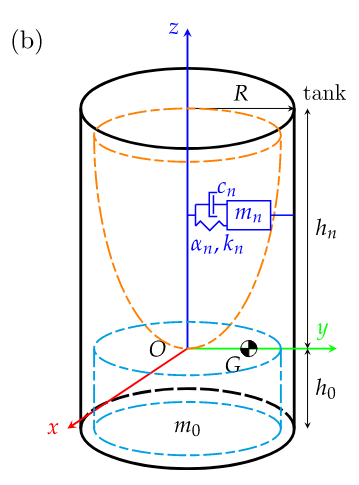
\includegraphics[width=0.5\textwidth]{images/sloshing_visualisation.png}
  \caption{sketch stolen from Viet et al. \cite{viet_antisloshing_2024}}
\end{figure}

conservation of mass equates to:

\begin{equation}
m_F = m_0 + \sum_{n=1}^{\inf} m_n
\end{equation}

the natural frequency of the sloshing motion is given by:

\begin{equation}
\omega_{n}^{2} = \frac{g \xi_{1n}}{R}tanh\left(\xi_{1n} \frac{h}{R}\right)
\end{equation}

giving the n-th sloshing mass as:

\begin{equation}
m_n = m_F \frac{2R}{\xi_{1n}h(\xi_{1n}^2-1)}tanh\left(\xi_{1n} \frac{h}{R}\right)
\end{equation}

damping ratio:

\begin{equation}
\zeta_n = \frac{2.89}{\pi}\sqrt{\frac{\nu}{R^{3/2}g^{1/2}}}
\end{equation}

The sloshing mass moves along a parabolic surface, with an attached nonlinear spring exerts forces \(\alpha_n k_n x_{n}^{2w-1}\) and \(\alpha_n k_n y_{n}^{2w-1}\) in the \(x\) and \(y\) direction respectively and \(\alpha_n k_n r_{n}^{2w-1}\) in the radial direction for the radia generalised coordinate \(r_n\).

Parabolic surface's analytical formula:

\begin{equation}
z_n = \frac{\omega_{n}^{2}}{2g}(x_{n}^{2} + y_{n}^{2})
\end{equation}

Time derivative:

\begin{equation}
\dot z_n = \frac{\omega_{n}^{2}}{2g}(x_{n} \dot x_{n} + y_{n} \dot y_{n})
\end{equation}

EoM from Lagrange:

\begin{equation}
\begin{cases}
\begin{aligned}

\frac{d}{dt}\left(\frac{\partial \cmsyT}{\partial \dot x_n}\right) - \frac{\partial \cmsyT}{\partial x_n} + \frac{\partial \cmsyV}{\partial x_n} &= -\frac{\partial \cmsyD}{\partial \dot x_n} \\
\frac{d}{dt}\left(\frac{\partial \cmsyT}{\partial \dot y_n}\right) - \frac{\partial \cmsyT}{\partial y_n} + \frac{\partial \cmsyV}{\partial y_n} &= -\frac{\partial \cmsyD}{\partial \dot y_n} \\

\end{aligned}
\end{cases}
\end{equation}

\(\cmsyT\) being the kinetic energy of the nth sloshing mass 

\begin{equation}
\cmsyT = \frac{1}{2}m_n[(\dot x_0 + \dot x_n)^2 + (\dot y_0 + \dot y_n)^2 + \dot z_n^2] =  \frac{1}{2}m_n \left[(\dot x_0 + \dot x_n)^2 + (\dot y_0 + \dot y_n)^2 + \frac{\omega_n^4}{g^2}(x_n \dot x_n + y_n \dot y_n) \right]
\end{equation}

\(\cmsyV\) being the potential energy (gravity and non linear spring)

\begin{equation}
\cmsyV = m g z_n + \int_{0}^{r_n} \alpha_n k_n r_{n}^{2w - 1} d r_n = m g \frac{\omega_n^2}{2g}(x_n^2 + y_n^2) + \frac{\alpha_n k_n}{2w}(x_n^2 + y_n^2)^w
\end{equation}

\(\cmsyD\) is the energy dissipation based on Rayleigh

\begin{equation}
\cmsyD = \frac{1}{2} c_n (\dot x_n^2 + \dot y_n^2 + \dot z_n^2) = m_n \zeta_n \omega_n \left[\dot x_n^2 + \dot y_n^2 + \frac{\omega_n^2}{g}(x_n \dot x_n + y_n \dot y_n)\right] 
\end{equation}

Resulting EoM: 

\begin{equation}
\begin{cases}

(1 + \frac{\omega_n^4}{g^2}) \ddot x_n + \frac{\omega_n^4}{g^2} x_n y_n \ddot y_n + (2 \omega_n \zeta_n (1 + \frac{\omega_n^4}{g^2} x_n^2) + \frac{\omega_n^4}{g^2} x_n \dot x_n) \\ 
+ (2 \omega_n \zeta_n \frac{\omega_n^4}{g^2} x_n y_n + \frac{\omega_n^4}{g^2} x_n \dot y_n) \dot y_n + \omega_n^2 x_n (1+ \frac{\alpha_n}{R^2}(x_n^2 + y_n^2)) &= - \ddot x_0 
\\
\\
\frac{\omega_n^4}{g^2} x_n y_n \ddot{x_n} + (1 + \frac{\omega_n^4}{g^2} y_n^2) \ddot y_n + (2 \omega_n \zeta_n \frac{\omega_n^4}{g^2} y_n + \frac{\omega_n^4}{g^2} y_n \dot x_n) \dot x_n \\
+ (2 \omega_n \zeta_n(1+ \frac{\omega_n^4}{g^2} y_n^2) + \frac{\omega_n^4}{g^2} y_n \dot y_n) \dot y_n + \omega_n^2 y_n (1 + \frac{\alpha_n}{R^2}(x_n^2 + y_n^2)) &= - \ddot y_0 \\

\end{cases}
\end{equation}

the maximum sloshing height is given by:

\begin{equation}
\bar \eta_n = \frac{\xi_{1n}^2 h m_n}{m_F R} \sqrt{x_n^2 + y_n^2} = \frac{\xi_{1n}^2 h m_n}{m_F R}r_n
\end{equation}

simplification: the sum of the sloshing heights caused by the higher modes is negligible compared to the first mode. Therefore the free surface shape \(\eta(r,\theta)\) can be approximated by:

\begin{equation}
\bar \eta(r,\theta) = \sum_{n}^{} \bar \eta_n \frac{J_1(\xi_{1n}\frac{r}{R})}{J_1(\xi_{1n})} \cos(\theta) \approx \bar \eta_1 \frac{J_1(\xi_{1n}\frac{r}{R})}{J_1(\xi_{1n})}cos(\theta)
\end{equation}

dynamic equation of the sloshing model:

\begin{equation}
M(q) \ddot q + C(q, \dot q) \dot q + G(q) + D = Q u
\end{equation}

with:
\begin{equation}\label{eqk27aligned}
\begin{aligned}[b]
\mathbf{M}(\mathbf{q})
%
&= \begin{bmatrix}
(1 + \frac{\omega_n^4}{g^2} x_n^2) & \frac{\omega_n^4}{g^2} x_n y_n & 0 & 0 \\
\frac{\omega_n^4}{g^2} x_n y_n & (1 + \frac{\omega_n^4}{g^2} y_n^2) & 0 & 0 \\
0 & 0 & 1 & 0 \\
0 & 0 & 0 & 1 
\end{bmatrix};
\mathbf{q}
= \begin{bmatrix}
x_n \\
y_n \\
x_0 \\
y_0
\end{bmatrix};
\mathbf{u}
= \begin{bmatrix}
u_x \\
u_y 
\end{bmatrix}; \\
\mathbf{C}(\mathbf{q}, \dot{\mathbf{q}})
&= \begin{bmatrix}
2 \omega_n \zeta_n (1 + \frac{\omega_n^4}{g^2} x_n^2) + \frac{\omega_n^4}{g^2} x_n \dot x_n & 2 \omega_n \zeta_n \frac{\omega_n^4}{g^2} x_n y_n + \frac{\omega_n^4}{g^2} x_n \dot y_n & 0 & 0 \\
2 \omega_n \zeta_n \frac{\omega_n^4}{g^2} x_n y_n + \frac{\omega_n^4}{g^2} y_n \dot x_n & 2 \omega_n \zeta_n (1 + \frac{\omega_n^4}{g^2} y_n^2) + \frac{\omega_n^4}{g^2} y_n \dot y_n & 0 & 0 \\
0 & 0 & 0 & 0 \\
0 & 0 & 0 & 0
\end{bmatrix}; \\
\mathbf{G}(\mathbf{q})
&= \begin{bmatrix}
\omega_n^2 x_n (1 + \frac{\alpha_n}{R^2}(x_n^2 + y_n^2)) \\
\omega_n^2 y_n (1 + \frac{\alpha_n}{R^2}(x_n^2 + y_n^2)) \\
0 \\
0
\end{bmatrix};
\mathbf{Q}
= \begin{bmatrix}
-1 & 0 \\
0 & -1 \\
1 & 0\\
0 & 1
\end{bmatrix}
\end{aligned}
\end{equation}

\section{Robotics}
\label{sec:robotics}

\subsection{Manipulator}
\label{sec:robotics:manipulator}

Goal of the laboratory is to use one or more 6 or 7 DOF manipulators for basic and advanced laboratory tasks. 

Modeling a robot involves studies about its kinematic behavior, namely the forces needed to produce a certain motion. This provides a description of how the links of the robot move in relation to each other. Two problems arise: the direct and inverse kinematics problem. The direct kinematics problem is to find the position and orientation of the end effector given the joint angles. The inverse kinematics problem is to find the joint angles given the position and orientation of the end effector. For serial Robots, like 6 DOF arms, the inverse kinematics problem is more complex than the direct kinematics problem. 

\subsubsection{Canidates}
\begin{itemize}
  \item KUKA LBR iiwa 7 R800
  \item UR7e - force-moment-sensor only in the gripper, joint torque mode ?
  \item Franka Reaserch 
  \item Kinova Gen3
  \item Flexiv Rizon - direct force control
\end{itemize}

\subsection{Platform}
\label{sec:robotics:platform}

\subsection{sensors}
\label{sec:robotics:sensor}

\subsubsection{Tracking System}
\label{sec:robotics:sensor:tracking_system}

Camera solution for tracking the area of operation. Mostly done by triangulation of a point via multiple cameras. Common systems are provided by :
\begin{itemize}
  \item Vicon
  \item OptiTrack
  \item Qualisys
\end{itemize}

\subsubsection{Camera System}
\label{sec:robotics:sensor:camera_system}

Robot endeffector mounted cameras for tracking the environment. Can be used for object detection and tracking, as well as for navigation. There different classes of cameras:
\begin{itemize}
  \item RGB cameras
  \item Depth cameras
    \begin{itemize}
      \item Basler ToF
    \end{itemize} 
  \item LIDAR
\end{itemize}

\subsection{Enviroment}
\label{sec:robotics:enviroment}

\subsection{Simulation}
\label{sec:robotics:simulation}
Simulation of robotics behaviour is done primarily in the Gazebo simulator. The simulation is based on the Robot Operating System (ROS) and uses the ROS control framework to simulate the robot's behavior. As an alternative Simulation enviroment NVIDIA Isaac Sim is being considered.

\subsubsection{Gazebo}
\label{sec:robotics:simulation:gazebo}

Gazebo Sim is a widely used open source simulation enviroment. There is already lots of ROS2 support. This makes for a good starting point for the simulation of the robotic enviroment. Gazebo is available on local hardware and can be used without any special requirements. 

Trajectory planning through the ROS2 MoveIt! package is possible.

\subsubsection{NVIDIA Isaac Sim}
\label{sec:robotics:simulation:nvidia_isaac_sim}

Isaac Sim, due to its NVIDIA grafics driver requirement is (atm) only functional on the DPE workstation. The usage is therefor not as straight forward as Gazebo, which is available on local hardware. To access the NVIDIA Isaac Sim enviroment, one must first connect to the server via SSH ('username'@172.22.64.245). Adress the Gitlab repository at \url{https://gitlab.kit.edu/kit/mvm/dpe/it/server-config} for more detailed Information on how exactly to run Isaac sim. 

Inside of the Isaac Sim Container, the enviroment needs to be set up. Namely the RWM and the path to the ROS2 bridge need to be set. Without the ROS2 bridge library path specification, the ROS2 bridge can not (easily?) be used in Isaac Sim.

\begin{lstlisting}[language=bash]
  export RMW_IMPLEMENTATION=rmw_cyclonedds_cpp
  export LD_LIBRARY_PATH=$LD_LIBRARY_PATH:/isaac-sim/exts/isaacsim.ros2.bridge/humble/lib
\end{lstlisting}

For ROS2 Communication the ROS2 Container has to be on the same network as the Isaac Sim Container. If this is not done due to the setup, the ROS2 Container can be started with the network attribute as follows:

Current implimention works with "ROS2 subscribe joint state" and a articulation controller for the prismatic joint. to set a position via ROS2 topic, one can use a bash command in the ROS2 enviroment:

\begin{lstlisting}[language=bash]
  export RMW_IMPLEMENTATION=rmw_cyclonedds_cpp
  export LD_LIBRARY_PATH=$LD_LIBRARY_PATH:/isaac-sim/exts/isaacsim.ros2.bridge/humble/lib
\end{lstlisting}


\begin{lstlisting}[language=bash]
  docker run -it --network=host "ROS2_Container"
\end{lstlisting}
e.g. in current implementation (plus mounting the a local directory to the container):
\begin{lstlisting}[language=bash]
ros2 topic pub /prismatic_joint/joint_command sensor_msgs/msg/JointState "
name: ['PrismaticJoint']
position: [-0.5]
"
\end{lstlisting}

\section{Tasks and inspiration}
\label{sec:tasks}
Sloshing free liquid transport. In extension supression of sloshing in multiple containers at once. Further tasks are to be determined, but are likely based on the usecase of the biological laboratory. Therefore sample preperation, transport and analysis are possible future tasks.

\url{https://umi-gripper.github.io/}


\section{Control}
\label{sec:Control}
First implimentions will make use of \textbf{Feed Forward Control}. with proper modeling of the Fluid behavior this control method should be sufficient to supress sloshing in the containers if the initial state of the fluid is known eg. at rest. 

One goal is the usage of a \textbf{Closed Loop Control}. Possible methods might be basic \textbf{PID}, \textbf{model predictive control}. One of the main issues lies within the measurement of the output. For many tasks the output is neither well defined nor easily measurable. Therefore the control system has to be able to handle a large amount of uncertainty. Eg. in the case of sloshing control, the shape of the freed surface is very hard to measure. Finding alternative outputs of the system and using state estimation methods might be an option. 

\subsection{ROS2}
\label{sec:Control:ROS2}

ROS2 is the second generation of the Robot Operating System. It is a set of software libraries and tools that help you build robot applications. ROS2 is designed to be more flexible, scalable, and secure than its predecessor. It supports multiple programming languages, including C++ and Python, and provides a rich set of libraries for various tasks such as perception, control, and planning. Best suited for R\&D and prototyping, but also used in industrie, military, and more.

most active version is ROS2 Humble Hawksbill, which is based on Ubuntu 22.04 LTS. Newest version at the writing of this document is ROS2 Jazzy, which is based on Ubuntu 24.04 LTS. 

\subsection{Industrial}
EtherCAT (by ETG) is mostly used for robotics in industrial settings. Combines ease of use of Ethernet with the speed and low latency of fieldbus systems.




\printbibliography
\end{document}

